\documentclass{proc}

\usepackage[utf8]{inputenc}
\usepackage[german]{babel}
\usepackage{graphicx}
\usepackage{hyperref}

\title{FeatureExtractor\\Kurzanleitung}
\author{Version 1.0}
\date{20. September 2016}

\begin{document}
	\maketitle
	\tableofcontents
	
%	\clearpage
	
	\section{Grunds"atzliches} 
	
	Das Tool \textit{FeatureExtractor} ist eine Java-Anwendung zur Identifikation von Technologie-Features in existierenden Softwaresystemen.
	Die GUI-Anwendung erm"oglicht dabei die Anlage und Verwaltung einer Wissensbasis (Architekturwissen) als Grundlage der Analyse.
	Zus"atzlich zur Bestimmung genutzter Features bietet das Tool die M"oglichkeit anhand der Wissensbasis potentiell sinnvolle Alternativen zu bestimmen.
	Ebenso ist eine Fokussierung auf m"ogliche Entscheidungspunkte vorgesehen.
	\\
	Die Anwendung trennt dabei die einzelnen fachlichen Komponenten voneinander und erm"oglicht eine sukzessive Ausf"uhrung einzelner Schritte im Prozess.
	
	\begin{figure}[h!]
		\centering
		\caption{Oberfl"ache \textit{FeatureExtractor}}
		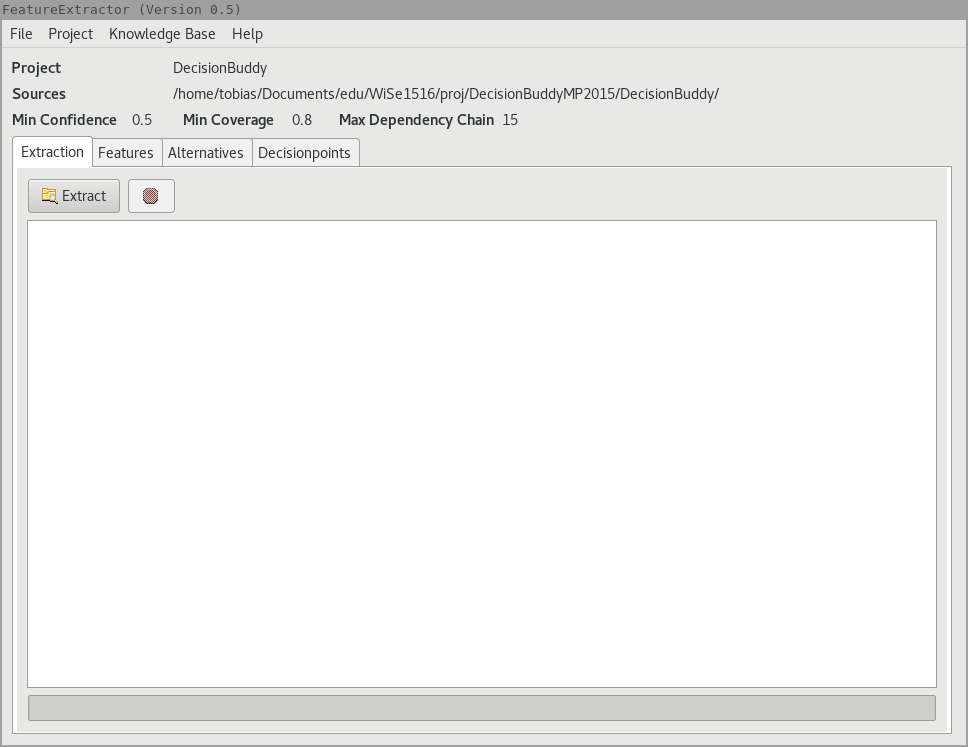
\includegraphics[width=0.5\textwidth]{../../80_images/screens/open.png}
	\end{figure}
	
	\section{Systemanforderungen}
	
	\begin{itemize}
		\item Betriebssystem: Windows, Linux, Mac
		\item Installation MySQL-Server (Version $\geq$ 5.0.11, getestet mit libmysql mysqlnd 5.0.11-dev)
		\item Installation Java 8 (Getestet mit OpenJDK Runtime Environment, Build 1.8.0\_102-b14)
%- SWT 4.5 (Provided)
	\end{itemize}
	
	\section{Installation}
	
	\begin{enumerate}
		\item Importierten Sie das mitgelieferte MySQL-Datenbank-Abbild.
		Es enth"alt die Grundstruktur der Datenbank sowie einige grunds"atzliche Inhalte.
		\item Extrahieren Sie das Archiv \texttt{featureextractor\_\textless{VERSION}\textgreater.zip}  an einen Ort ihrer Wahl.
		Stellen Sie sicher, das die Unterverzeichnisse \texttt{resources} sowie \texttt{config} im selben Ordner wie die entpackte \texttt{.jar}-Datei liegen.
		\item "Offnen sie die Datenbank-Konfigurationsdatei unter \texttt{config > database.properties} mit einem Text-Editor.
		Tragen Sie die Konfiguration ihrer lokalen MySQL-Datenbank ein.
		Die Konfiguration erwartet folgende Einstellungen:
		
		hibernate.connection.url=jdbc:mysql://\textless{URL}\textgreater\\
		hibernate.connection.username=\textless{USER}\textgreater\\
		hibernate.connection.password=\textless{PASSWORD}\textgreater\\
		\\
		\textless{URL}\textgreater{ } erwartet die Adresse der lokalen MySQL-installation. \textless{USER}\textgreater{ } sowie
		\textless{PASSWORD}\textgreater{ } erwarten Benutzername sowie Password der Installation.
		Diese muss f"ur den Zugriff eingerichtet sein.	
		\item Starten Sie das Tool, indem sie das Startskript \texttt{run.sh} (Linux, Mac) ausf"uhren, oder die \texttt{.jar}-Dateiausf"uhren.
	\end{enumerate}
	
	\subsection{Datenquelle}
	
	Grundlage der Wissensbasis ist eine MySQL-Datenbank.
	In dieser wird das genutzte Architekturwissen strukturiert hinterlegt und verwaltet.
	Eine manuelle Manipulation der Tabellen ist grunds"atzlich m"oglich, jedoch nicht empfehlenswert, da diese die Konsistenz der Datenstrukturen gef"ahrdet.
	Zur Manipulation ist ausschlie"slich die Oberfl"ache der Anwendung zu nutzen.
	Dies stellt sicher, das Abh"angigkeiten zwischen Datens"atzen und fachliche Komponenten gew"ahrleistet werden k"onnen.
	
	\subsection{Konfiguration}
	
	\begin{figure}[h!]
		\centering
		\caption{Konfiguration}
		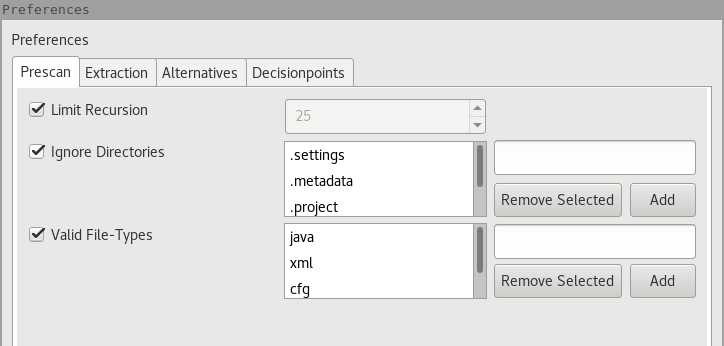
\includegraphics[width=0.5\textwidth]{../../80_images/screens/preferences.png}
	\end{figure}
	
	Unter \texttt{File > Preferences} finden sich einige Einstellungen, welche das Verhalten des Tools beeinflussen.
	In mehreren Reitern finden sich neben allgemeinen Einstellung vor allem Anpassungen f"ur die einzelnen Arbeitsschritte im Analyseprozess.
	Diese k"onnen zumeist durch Selektieren der jeweiligen Checkbox aktiviert bzw. deaktiviert werden.
	\\
	Zu beachten ist, dass entsprechende Einstellungen nur zur Laufzeit gespeichert werden und nach dem Neustart der Anwendung erneut justiert werden m"ussen.
	Nicht jede Einstellung ist tats"achlich implementiert.
	Weitere, nicht verf"ugbare Men"upunkte sind entsprechend ausgegraut dargestellt.
	
	\section{Verwaltung von Architekturwissen}
	
	Um die Konsistenz des Datenbestandes sicherzustellen, kann das genutzte Architekturwissen direkt im Tool verwaltet werden.
	Unter \texttt{Knowledge Base > View Structure} kann das aktuell hinterlegte Architekturwissen eingesehen werden.
	Die Ansicht beinhaltet alle Abh"angigkeiten innerhalb der Baumstruktur.
	Durch ein Aufklappen der einzelnen Knoten k"onnen untergeordnete Elemente eingesehen werden.
	Diese beinhalten Technologien, deren Features sowie, auf unterster Ebene, Indikatoren.
	
	\begin{figure}[h!]
		\centering
		\caption{"Uberblick Architekturwissen}
		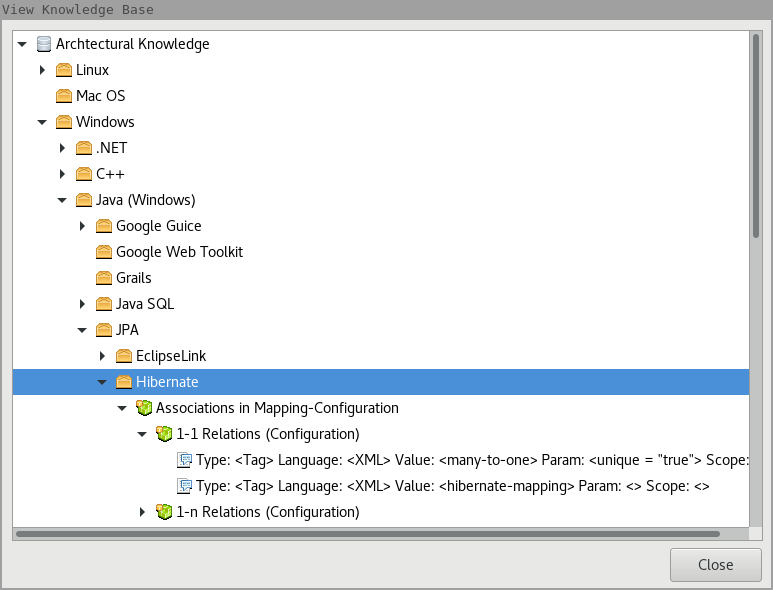
\includegraphics[width=0.5\textwidth]{../../80_images/screens/ak_view.png}
	\end{figure}
	
	\subsection{Features}
	
	Die Verwaltung einzelner Daten-Objekte im Architekturwissen erfolgt auf separaten Oberfl"achen.
	Einzelne Objekte k"onnen referenziert werden, um Abh"angigkeiten, Beziehungen und weitere Zusammenh"ange zu modellieren.
	\\
	Oberfl"achen zum Editieren von Datens"atzen sind grunds"atzlich "ahnlich aufgebaut.
	Sie enthalten jeweils eine tabellarische Darstellung aller vorhandenen Datens"atze.
	Je Spalte stellt sich ein Datensatz dar.
	Durch Auswahl dieses Datensatzes werden dessen Daten in die Felder unterhalb der Tabelle eingetragen.
	Innerhalb dieser Felder k"onnen sie editiert werden.
	Ein Druck auf \texttt{Confirm} "ubernimmt die "Anderungen an diesem Datensatz, speichert sie jedoch nicht nicht in der Datenbank.
	Ein Druck auf \texttt{Delete} l"oscht den Datensatz.\\
	Oberhalb der Tabelle kann ein neuer Datensatz angelegt werden.
	Dieser muss ebenfalls im unteren Abschnitt editiert und best"atigt werden.
	\\
	Ein Druck auf \texttt{Save} best"atigt die in dem aktuellen Fenster get"atigten "Anderungen und schreibt diese in die Datenbank.
	\texttt{Cancel} bricht den Vorgang ab und revidiert die "Anderungen.
	
	\begin{figure}[h!]
		\centering
		\caption{Verwaltung abstrakter Features}
		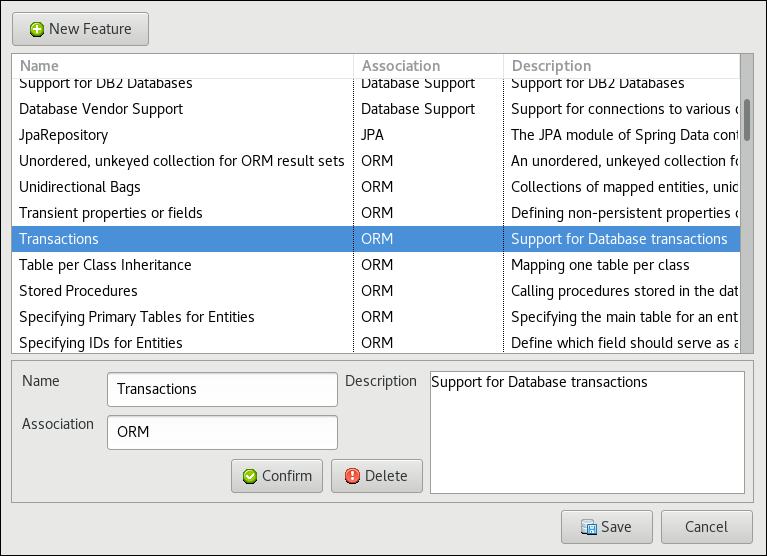
\includegraphics[width=0.5\textwidth]{../../80_images/screens/ak_edit_features.png}
	\end{figure}
	
	\subsection{Technologien}
	
	Parallel sind Technologien zu verwalten.
	Hier m"ussen anhand von Comboboxen zur Verkn"upfung von Abh"angigkeiten mehrere Technologien verbunden werden.
	\\
	Ein Druck auf \texttt{Edit Features} nach Auswahl Technologie "offnet einen Dialog zur Bearbeitung der dieser zugeordneten Technologie-Features.
	
	\begin{figure}[h!]
		\centering
		\caption{Verwaltung von Technologien}
		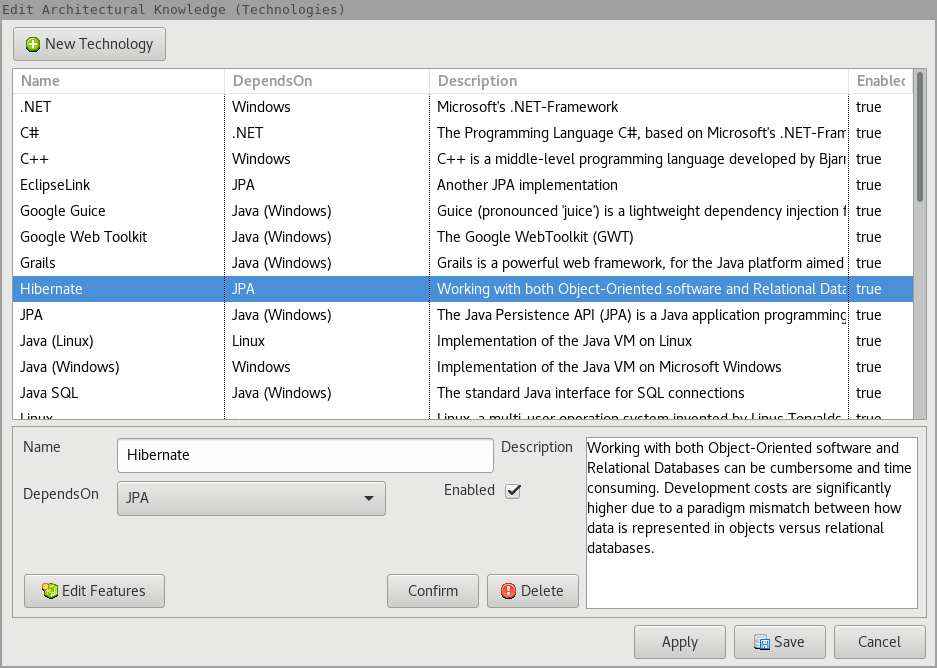
\includegraphics[width=0.5\textwidth]{../../80_images/screens/ak_edit_technologies.png}
	\end{figure}
	
	\subsection{Technologie-Features}
	
	Je Technologie wird eine eigene Menge von Technologie-Features verwaltet.
	Der entsprechende Dialog zeigt somit lediglich die Features der ausgew"ahlten Technologie.
	Pro Features k"onnen Indikatoren sowie ASTAs f"ur das ausgew"ahlte Feature bearbeitet werden.
	Ebenso k"onnen Abh"angigkeiten zu anderen Features modelliert werden.
	
	\begin{figure}[h!]
		\centering
		\caption{Verwaltung von Technologie-Features}
		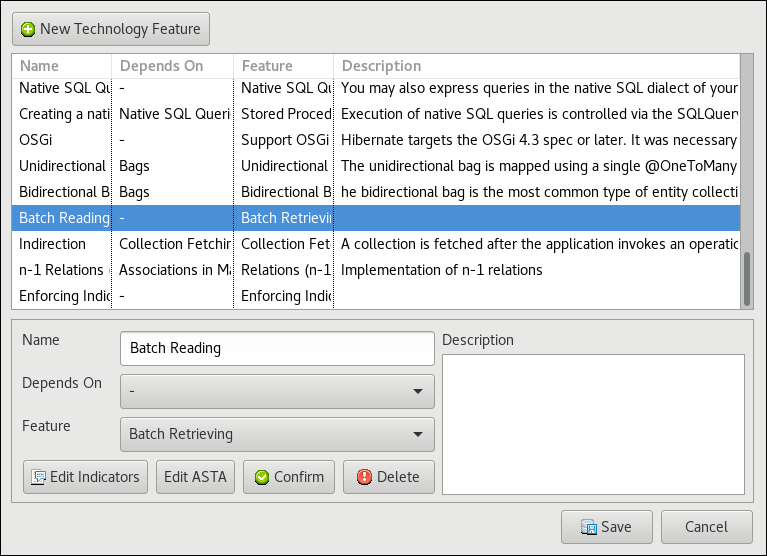
\includegraphics[width=0.5\textwidth]{../../80_images/screens/ak_edit_technology_features.png}
	\end{figure}
	
	\subsection{Indikatoren}
	
	Die Bearbeitung von Indikatoren legt die Gesamtheit aller charakteristischen Eigenschaften f"ur das ausgew"ahlte Feature fest.
	Anhand der auszuw"ahlenden Parameter kann jeder Indikator angepasst werden.
	
	\begin{figure}[h!]
		\centering
		\caption{Verwaltung von Indikatoren}
		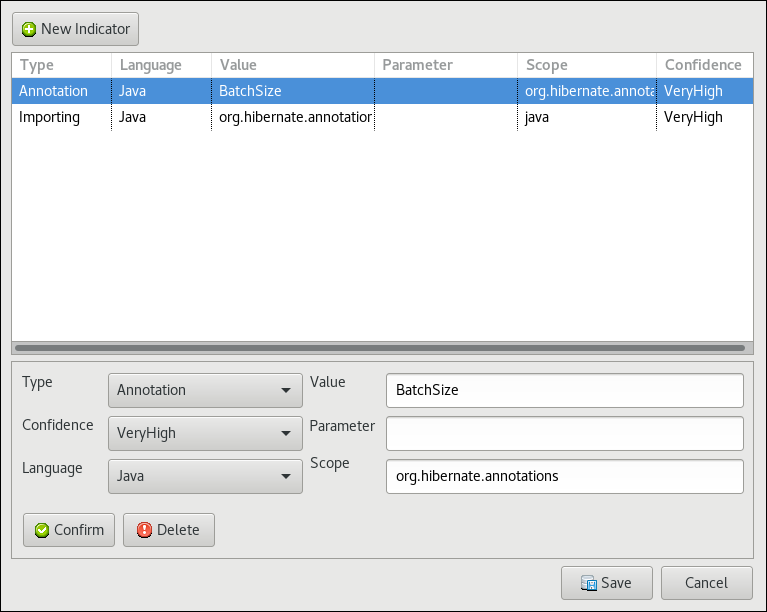
\includegraphics[width=0.5\textwidth]{../../80_images/screens/ak_edit_indicators.png}
	\end{figure}
	
	\subsection{ASTAs}
	
	Paralleles gilt f"ur die Modellierung \textit{Architecturally Significant Technology Aspects} (ASTAs).
	Diese dienen im sp"ateren Prozess der Anreicherung von Information und sind entsprechend wenig formalisiert.
	Es bestehen keine Beziehungen zu anderen Objekten.
	
	\begin{figure}[h!]
		\centering
		\caption{Verwaltung von ASTAs}
		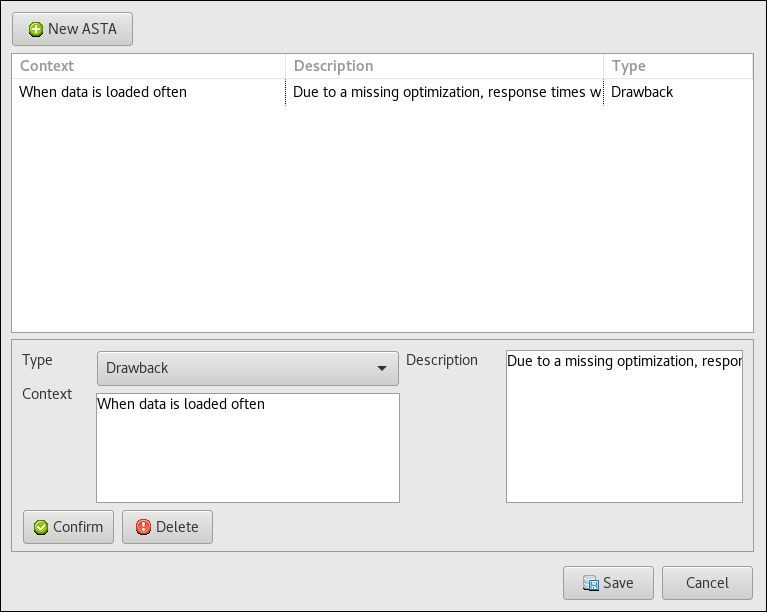
\includegraphics[width=0.5\textwidth]{../../80_images/screens/ak_edit_asta.png}
	\end{figure}
	
	\section{Projekte}
	
	Um Softwaresystem zu analysieren, fasst der \textit{FeatureExtractor} notwendige Informationen als \textit{Projekte} zusammen.
	Diese beinhalten lediglich den (lokalen) Speicherort der zu analysierenden Quellcodedateien sowie die spezifischen Einstellungen f"ur Grenzwerte und maximale L"ange des Abh"angigkeitspfades.
	Zus"atzlich werden Teile der Ergebnisse projektbezogen in der Datenbank gespeichert.
	
	\subsection{Projekt "offnen}
	
	"Uber \texttt{File > Open Project...} kann ein Projekt ge"offnet werden.
	Die Auswahl zeigt alle in der Datenbank gespeicherten Projekte an.
	Der Name eines Projektes ist nicht zwangsl"aufig einzigartig, da etwa auch Untermengen eines Systems betrachtet werden k"onnen.
	Die Wahl eines sinnvollen Bezeichners ist zu empfehlen.
	
	\begin{figure}[h!]
		\centering
		\caption{"Offnen eines Projektes}
		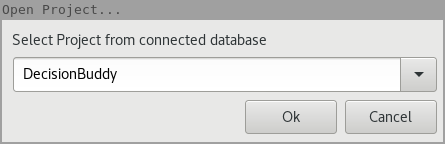
\includegraphics[width=0.5\textwidth]{../../80_images/screens/project_open.png}
	\end{figure}
		
	\subsection{Projekt anlegen}
	
	Mittels \texttt{File > New Project...} kann ein neues Projekt angelegt werden.
	Zu diesem Zweck m"ussen Name und Pfad der zu analysierenden Quellcodedateien gew"ahlt werden.
	Zudem m"ussen gegebenenfalls die Einstellungen f"ur die Schwellwerte bez"uglich Konfidenz und Abdeckungsrate, sowie die maximale L"ange des Abh"angigkeitspfades angepasst werden.
	Tooltips informieren "uber die Verwendung dieser Werte im weiteren Verlauf der Analyse.
	
	\begin{figure}[h!]
		\centering
		\caption{Anlegen eines Projektes}
		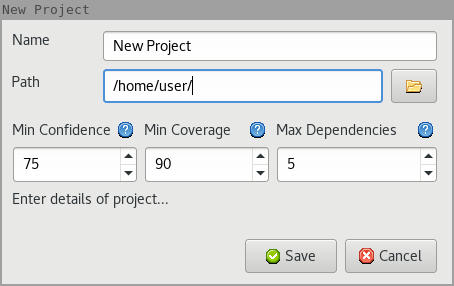
\includegraphics[width=0.5\textwidth]{../../80_images/screens/project_new.png}
	\end{figure}
	
	\subsection{Projekt bearbeiten}
	
	Bei Anlage eines Projektes justierte Schwellwerte und Einstellungen sind nicht final.
	Sie k"onnen mittels des unter \texttt{Project > Edit...} verf"ugbaren Dialoges nachtr"aglich angepasst werden und wirken sich unmittelbar auf die Folgenden Arbeitsschritte aus.
	Bereits hinterlegte Ergebnisse werden erst bei erneuter Durchf"uhrung "uberschrieben.
	
	\begin{figure}[h!]
		\centering
		\caption{Bearbeiten eines Projektes}
		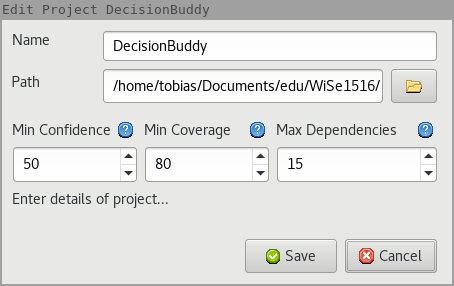
\includegraphics[width=0.5\textwidth]{../../80_images/screens/project_edit.png}
	\end{figure}
	
	\section{Analyse}
	
	Die Oberfl"ache des \textit{FeatureExtractor} zergliedert sich grunds"atzlich in zwei Bereiche.
	Im oberen Bereich finden sich Informationen zum aktuell geladenen Projekt.
	Eingestellte Grenzwerte sind hier einzusehen.
	\\
	Im unteren Bereich findet sich die eigentliche Arbeitsoberfl"ache.
	In Form mehrerer Reiter sind die einzelnen Arbeitsschritte angeordnet.
	Unterteilt wird dabei zwischen Extraktion, Extrahierte Features, Alternativen und Entscheidungspunkten.
	
	\subsection{Extraktion}
	
	Der Reiter \texttt{Extraction} beinhaltet die eigentliche Extraktion von Technologie-Features aus dem durch das Projekt vorgegebene Softwaresystem.
	Im oberen Bereich stellen sich die Schaltfl"achen \texttt{Extract} sowie \texttt{Abort} dar.
	Sie starten bzw. stoppen den Extraktionsprozess f"ur das ausgew"ahlte Projekt.
	Letzteres ist sinnvoll, da der Extraktionsprozess potentiell viel Zeit in Anspruch nehmen kann.
	\\
	Unmittelbar unter den Schaltfl"achen befindet sich die Ausgabe des Prozesses.
	Sie informiert detailliert "uber den Fortschritt der Extraktion.
	\\
	Ein Fortschrittsbalken zeigt unterhalb den Fortschritt an.
	Ein Tooltip gibt Aufschluss dar"uber, wieviele Elemente bereits verarbeitet wurden.
	
	\begin{figure}[h!]
		\centering
		\caption{Extrahieren von Technologie-Features}
		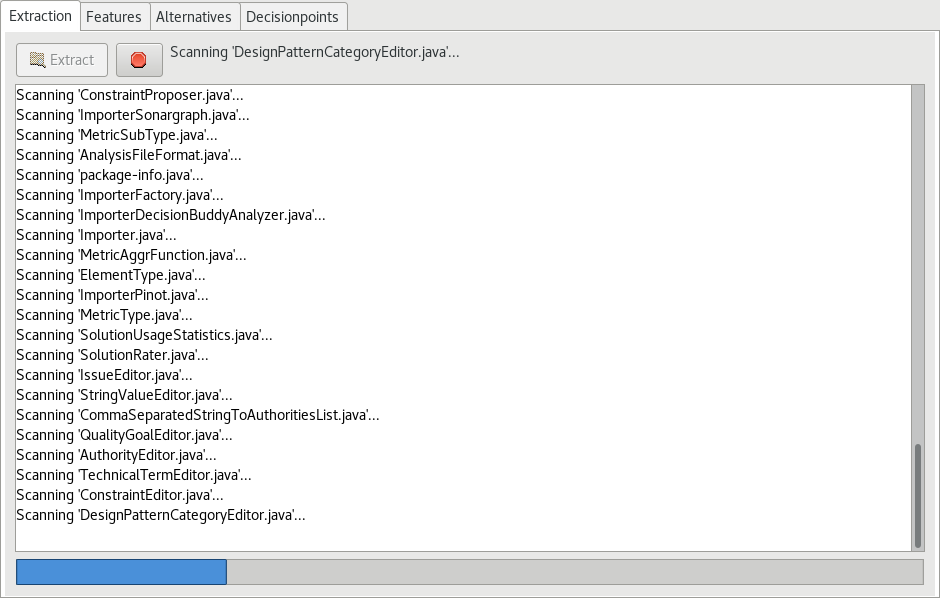
\includegraphics[width=0.5\textwidth]{../../80_images/screens/process_extract.png}
	\end{figure}
	
	\subsection{Extrahierte Features}
	
	Der Reiter \texttt{Features} zeigt in Folge die extrahierten Technologie-Features.
	Ein Druck auf die Schaltfl"ache \texttt{Load} l"adt die Ergebnisse aus der Datenbank.
	In diesem Schritt werden die lose zusammenh"angenden Ergebnisse aggregiert und f"ur die Darstellung als Baumstruktur verarbeitet.
	Das Laden der Ergebnisse kann in diesem Schritt einige Zeit in Anspruch nehmen und h"angt mit der Speicherung der Ergebnisse zusammen.
	Diese ist vorrangig f"ur die weitere Verarbeitung optimiert.
	Die Darstellung der Ergebnisse ist optional.
	\\
	Ergebnisse werden analog der Ordnerstruktur des analysierten Verzeichnisses dargestellt.
	Einzelne Elemente werden anhand ihres Dateinamens dargestellt.
	Bei Auswahl eines Elemente zeigt der untere Abschnitt der Anzeige die in diesem Kontext extrahierten Technologie-Features inklusive der bestimmten Konfidenz.
	Bei Auswahl eines Paketes werden die in diesem und seinen Unterpaketen extrahierten Features aggregiert.
	
	\begin{figure}[h!]
		\centering
		\caption{Extrahierte Technologie-Features}
		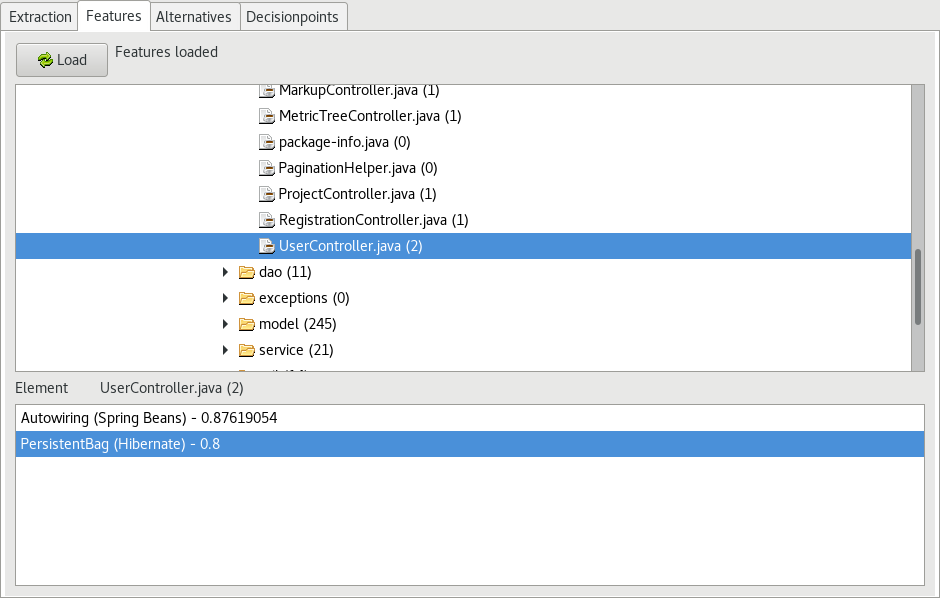
\includegraphics[width=0.5\textwidth]{../../80_images/screens/process_results.png}
	\end{figure}
	
	\subsection{Bestimmen von Alternativen}
	
	Auf dem Reiter \texttt{Alternatives} ist die Bestimmung von Alternativen durchzuf"uhren.
	Dies geschieht durch einen Druck auf die Schaltfl"ache \texttt{Find}.
	Voraussetzung ist daf"ur, dass f"ur das ausgew"ahlte Projekt zun"achst Technologie-Features extrahiert wurden.
	\\
	Der Reiter zeigt im oberen Abschnitt die eingesetzten Technologien an.
	Die Auswahl einer dieser Technologien zeigt folgend im unteren Abschnitt deren eingesetzte Features sowie m"ogliche Alternativen an.
	\\
	Die hier dargestellte Abdeckungsmatrix stellt alle Alternativen sowie die momentan genutzten Features "ubersichtlich zusammen.
	In der linken Spalte werden momentan genutzte Features aus der ausgew"ahlten Technologie gelistet.
	Rechts von dieser stellen sich alle potentiellen Alternativen dar.
	Der Kopf der Spalte indiziert jeweils den Namen der Technologie, ebenso die Abeckungsrate.
	In jeder Zeile findet eine Gegen"uberstellung der von einzelnen Technologien implementierten Features statt.
	Implementiert eine Technologie ein genutztes Feature ebenfalls, ist die entsprechende Zelle mit einem \texttt{X} markiert.
	Wird das Feature nicht umgesetzt, mit einem \texttt{O}.
	
	\begin{figure}[h!]
		\centering
		\caption{Abdeckungsmatrix}
		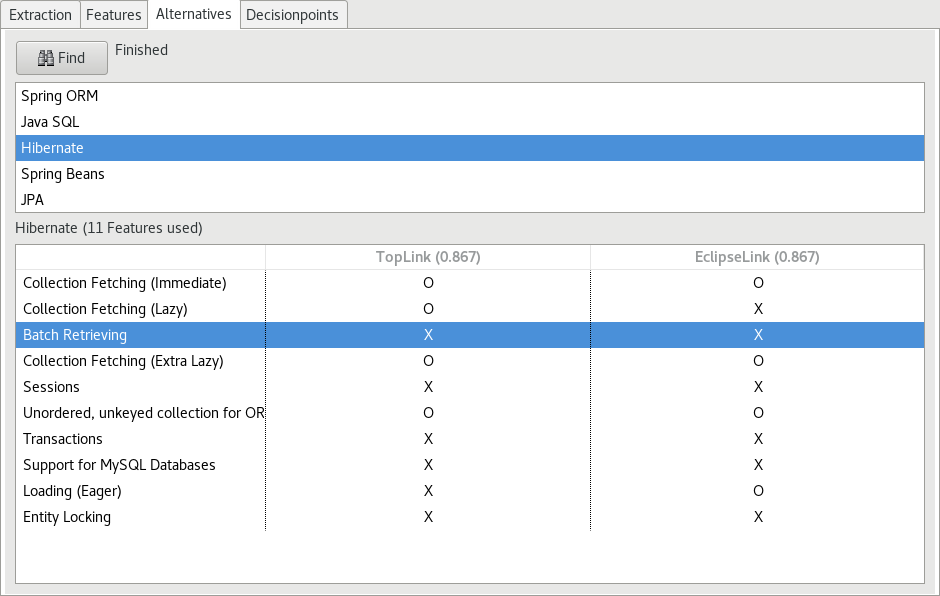
\includegraphics[width=0.5\textwidth]{../../80_images/screens/process_alternatives.png}
	\end{figure}
	
	Um die Auswahl einer geeigneten Alternative zu unterst"utzen k"onnen die ASTAs der jeweiligen Implementation konsultiert werden.
	Um diese anzuzeigen muss in der Zeile des jeweiligen Features nach Bet"atigung der rechten Maustaste die zu betrachtende Technologie ausgew"ahlt werden.
	Es "offnet sich ein Fenster, welches die relevanten ASTAs anzeigt.
	Mehrere Fenster k"onnen ge"offnet werden, um die ASTAs zu vergleichen.
	\\
	Konnten keine Alternativen bestimmt werden, k"onnen lediglich eingesetzte Features dargestellt werden.

	\begin{figure}[h!]
		\centering
		\caption{Betrachtung relevanter ASTAs}
		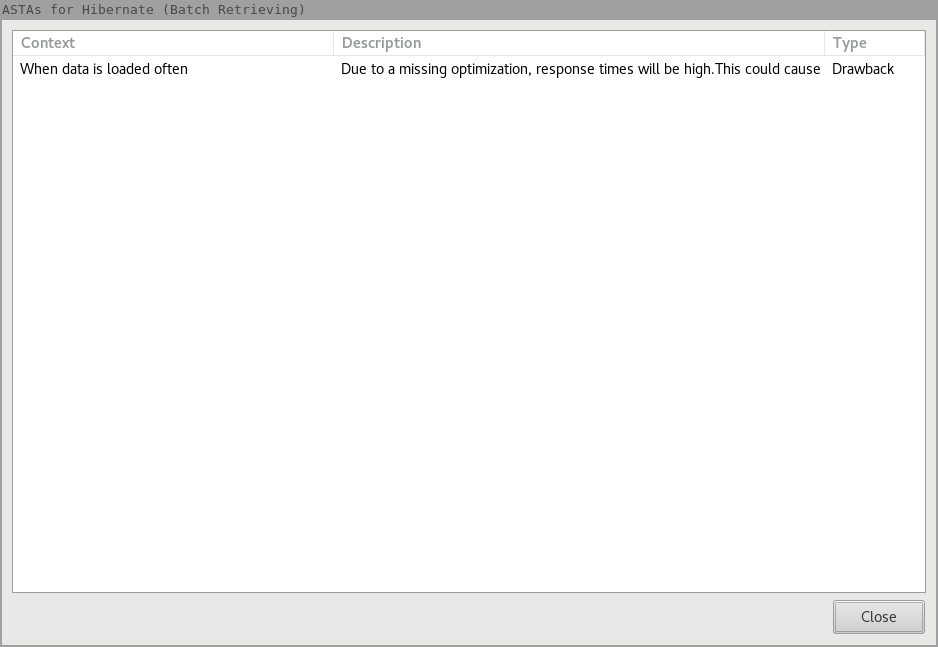
\includegraphics[width=0.5\textwidth]{../../80_images/screens/process_astas.png}
	\end{figure}
	
	\subsection{Bestimmen von Entscheidungspunkten}
	
	Der Reiter \texttt{Decisionpoints} dient der Bestimmung von Entscheidungspunkten.
	Durch einen Druck auf die Schaltfl"ache \texttt{Find} bestimmt das Tool diese.
	Pro Entscheidungspunkt werden entsprechend relevante Informationen aufgelistet.
	Ebenso wird die L"ange des Abh"angigkeitspfades dargestellt.
	Diese kann einen Einfluss auf die tats"achliche Entscheidung haben.
	Zudem wird bei niedrigen Abdeckungsraten ein Warnhinweis gegeben.
	Voraussetzung f"ur die Bestimmung von Entscheidungspunkten ist die vorherige Bestimmung von Alternativen.
	
	\begin{figure}[h!]
		\centering
		\caption{Entscheidungspunkte}
		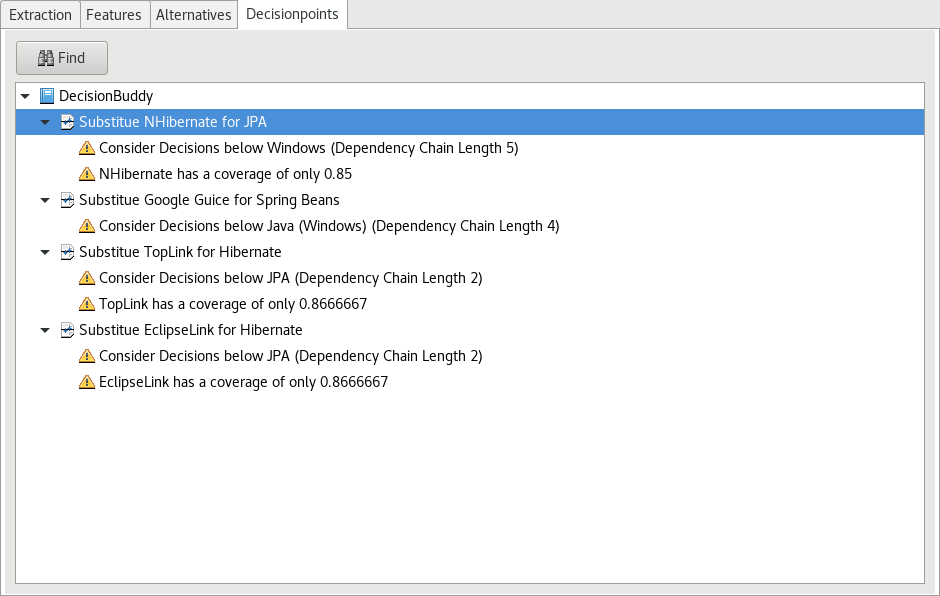
\includegraphics[width=0.5\textwidth]{../../80_images/screens/process_decision_points.png}
	\end{figure}
	
	\section{Bekannte Probleme}
	
	\begin{itemize}
		\item Die Nutzung von SWT kann auf Linux-basierten Systemen Probleme mit GTK3+ verursachen.
		Dies f"uhrt zu Abst"urzen beim Starten der Anwendung, vermutlich verursacht durch inkompatible Bibliotheken.
		Ein (tempor"ares) Deaktivieren der Nutzung von GTK3 kann allerdings Abhilfe schaffen.
		Das mitgelieferte Start-Skript (\texttt{run.sh}) "ubernimmt diese Aufgabe.
		F"ur weitere Informationen, siehe \url{https://www.eclipse.org/swt/faq.php\#gtkstartup}
		\item Auf einigen Systemen werden nicht alle oder keine der hinterlegten Icons angezeigt.
		Dies scheint mit der inkonsistenten Implementation der SWT-Bibliotheken zusammenzuh"angen.
		Eine fehlende Darstellung der Icons hat jedoch keinen Einfluss auf die Funktionalit"aten des Programmes.
		\item Unter MaxOS Cocoa kann es zu Problemen bei der Nutzung von SWT kommen. Standardm"a"sig startet Java die Anwendung in einem gesonderten Thread. Dies ist bei der Nutzung von SWT jedoch nicht erlaubt, da Steuerelemente im Haupt-Thread instantiiert werden m"ussen. Die Nutzung des Start-Skriptes (\texttt{run.sh}) umgeht diesen Sachverhalt.
	\end{itemize}
		
\end{document}